\documentclass[../paper.tex]{subfiles}
\begin{document}
\section{Эксперименты}
%
Для аналитического способа.

\begin{tabular}{ l l l l }
\hline
    Функция        & Способ вычисления                              & Машинная точность                     & Значение                  \\ 
                   &                                                & (размер мантиссы),                    &                           \\
\hline%%%%%%%%%%%%%%%%%%%%%%%%%%%%%%%%%%%%%%%%%%%%%%%%%%%%%%%%%%%%%%%%%%%%%%%%%%%%%%%%%%%%%%%%%%%%%%%%%%%%%%%%%%%%%%%%%%%%%%%%%%%%%%%%%%%%
    $g_{0,0}(1)$   & численно, интеграл,                            & 100 десятичных знаков                 & $ 0.864$                  \\
	           & контур $[1-100i, 1+100i]$                      &                                       &                           \\

	           & численно, ряд                                  & 256 двоичных знаков                   & $ 0.864$                  \\

    $g_{0,0}(10)$  & численно, интеграл                             & 100 десятичных знаков                 & $ 0.591$                  \\
                   & контур $[1-100i, 1+100i]$                      &                                       &                           \\

                   & численно, ряд                                  & 256 двоичных знаков                   & $ 0.591$                  \\

    $g_{0,0}(100)$ & численно, интеграл                             & 100 десятичных знаков                 & $-2 \times 10^{19}$       \\
	           & контур $[1-10i, 1+10i]$                        &                                       &                           \\
		   
                   & численно, ряд                                  & 256 двоичных знаков                   & $-0.440$                  \\
\hline
\end{tabular}

\bigskip

Для численного вычисления интеграла. Мы использовали шаг $0{,}1$ и $\alpha = 0{,}1$. И использовали $m=\{-5, \dots, 5\}$, $n=\{-5, \dots, 5\}$.

\begin{figure}[h]
	\begin{minipage}{0.48\textwidth}
		\centering
		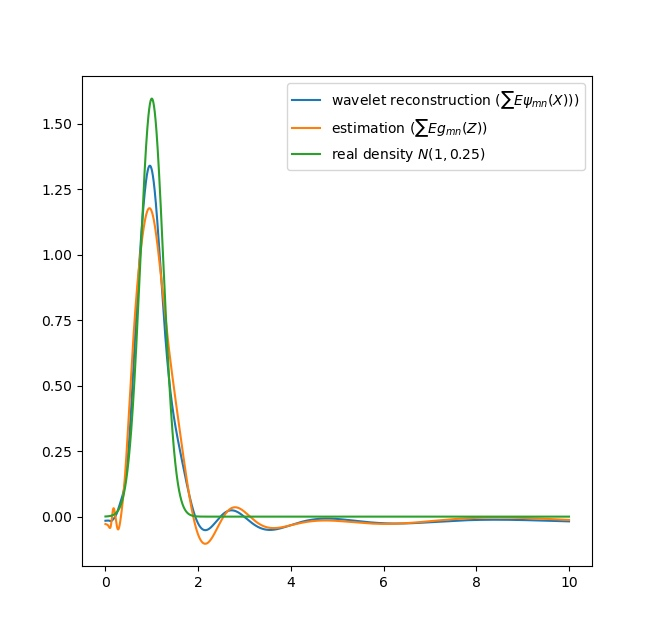
\includegraphics[width=\textwidth]{norm}
		\caption{$X \sim \mathcal{N}(0, 1)$}
	\end{minipage}\hfill
	\begin{minipage}{0.48\textwidth}
		\centering
		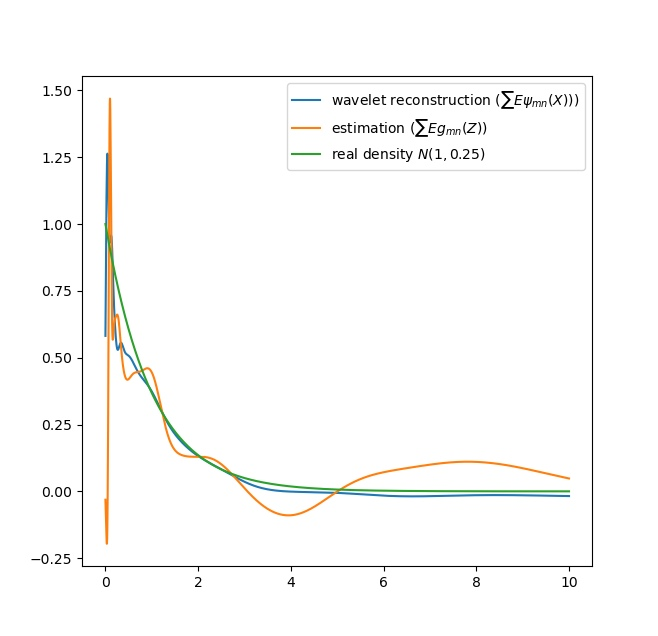
\includegraphics[width=\textwidth]{exp}
		\caption{$X \sim \exp(1)$}
	\end{minipage}\hfill
\end{figure}

\begin{figure}[h]
	\begin{minipage}{0.48\textwidth}
		\centering
		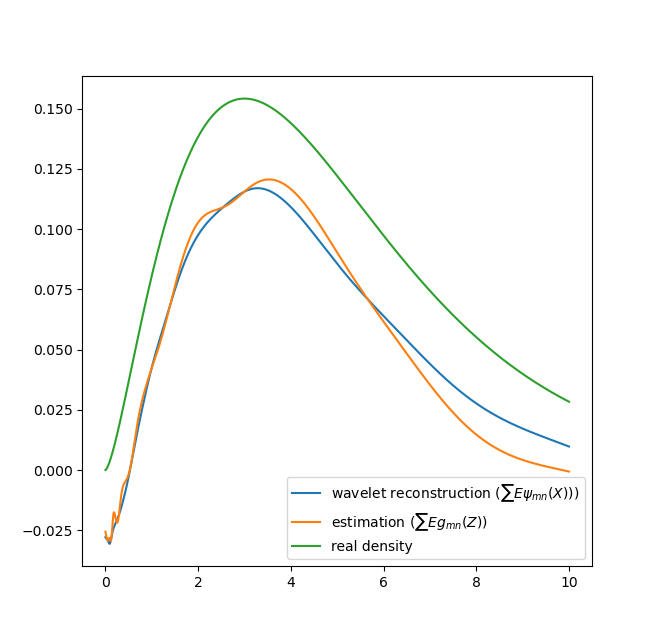
\includegraphics[width=\textwidth]{chisq}
		\caption{$X \sim \chi^2_5$}
	\end{minipage}\hfill
	\begin{minipage}{0.48\textwidth}
		\centering
		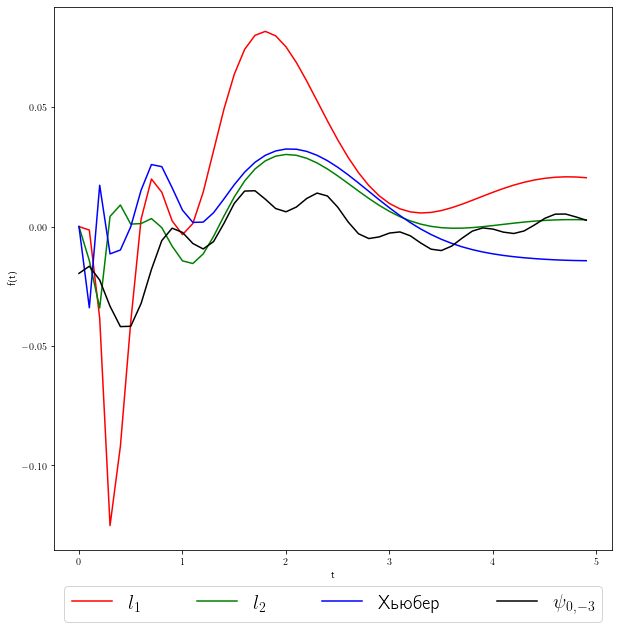
\includegraphics[width=\textwidth]{comp-loss}
		\caption{Сравнение функций ошибок для метода градиентного спуска}
	\end{minipage}\hfill
\end{figure}

\begin{figure}[h]
	\begin{minipage}{0.48\textwidth}
		\centering
		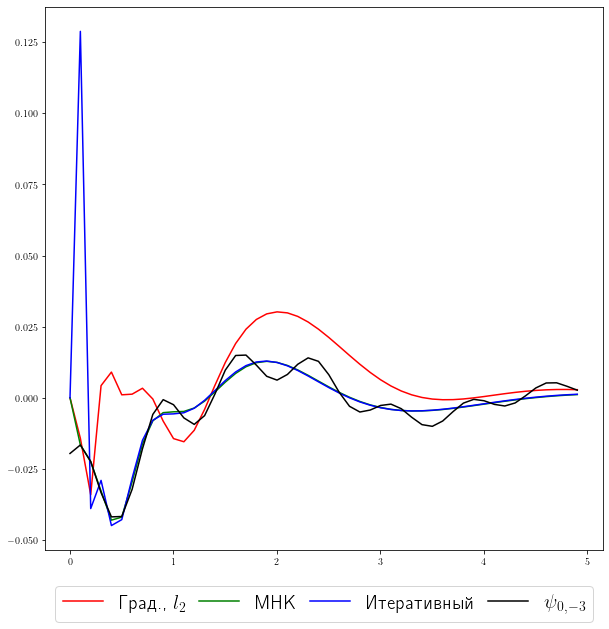
\includegraphics[width=\textwidth]{comp-method}
		\caption{Сравнение методов градиентного спуска, итеративного и МНК-оценки}
	\end{minipage}\hfill
	\begin{minipage}{0.48\textwidth}
		\centering
		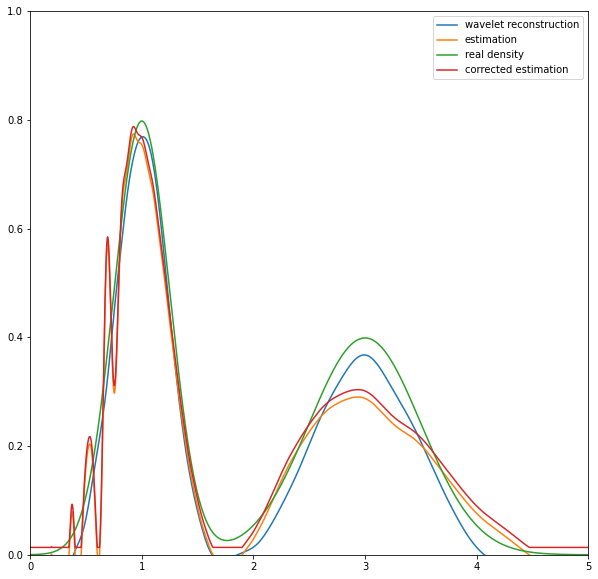
\includegraphics[width=\textwidth]{est-lse}
		\caption{МНК-оценка для смеси нормальных распределений}
	\end{minipage}\hfill
\end{figure}

\begin{figure}[h]
	\begin{minipage}{0.48\textwidth}
		\centering
		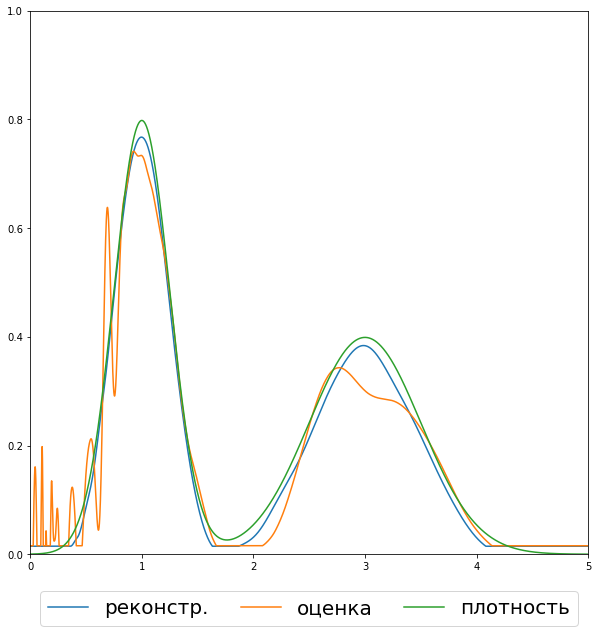
\includegraphics[width=\textwidth]{est-l2}
		\caption{Оценка методом градиентного спуска для смеси нормальных распределений}
	\end{minipage}\hfill
	\begin{minipage}{0.48\textwidth}
		\centering
		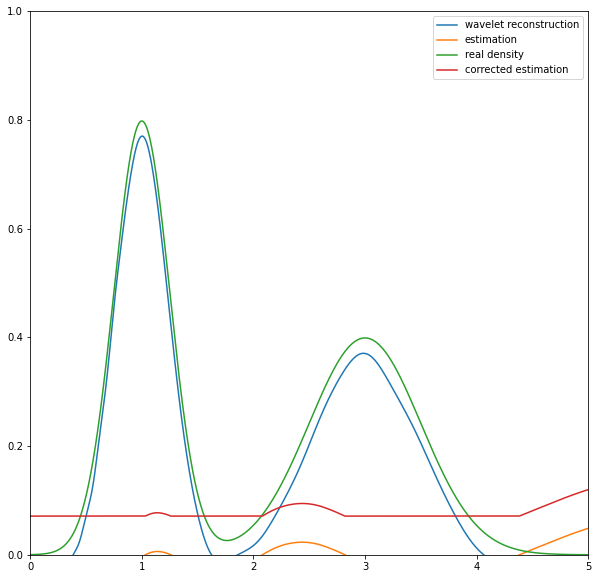
\includegraphics[width=\textwidth]{est-it}
		\caption{Оценка итеративным методом для смеси нормальных распределений}
	\end{minipage}\hfill
\end{figure}
\end{document}
